\documentclass{article}
\usepackage{babel}
\usepackage{derivative}
\usepackage{natbib}
\bibliographystyle{unsrtnat}
\usepackage{tabularx}
\usepackage{amsmath}
\usepackage{amssymb}
\usepackage{enumitem}
\usepackage{amsfonts}
\usepackage{physics}
\usepackage{dsfont}
\usepackage{tikz}
%\usetikzlibrary{quantikz2}%for quantum circuits
\usepackage{circuitikz}%for logic gates
\usepackage{caption}
\usepackage{graphicx}
\usepackage[left=20mm, right=20mm, top=20mm, bottom=20mm]{geometry}
\usepackage{cite}
\usepackage{mathrsfs}
\usepackage[most,many,breakable]{tcolorbox}
\renewcommand{\theequation}{\thesection.\arabic{equation}}
\makeatletter
\let\old@section\section
\def\section{\setcounter{equation}{0}\old@section}
\makeatother
\renewcommand{\tablename}{\textbf{Tabla}}
\renewcommand{\listfigurename}{\textbf{Figura}}
\usepackage[final]{hyperref}
\hypersetup{
 colorlinks=true,
 linkcolor=blue,       
 citecolor=blue,  
 filecolor=magenta,     
 urlcolor=blue         
}
\usepackage{titleps,kantlipsum}
\newpagestyle{mypage}{%
\headrule
\sethead{\MakeUppercase{\thesection\quad \sectiontitle}}{}{\thesubsection\quad \subsectiontitle}
\setfoot{}{}{\thepage}
}
\settitlemarks{section,subsection}
\pagestyle{mypage}
\input{~/Documents/Vim/Tex/Newcomm/theorem.tex}



\title{Ecuaciones para diapositivas}
\author{César Lévano}
\date{\today}

\begin{document}
\maketitle\newpage
\setcounter {page} {1}
\tableofcontents
\section{Resumen}
En este informe se muestran los resultados al analizar el campo magnético generado por dos bobinas de Helmholtz. Además  usando el valor del factor de calibración de las bobinas de Helmholtz y el cambio en la inclinación de la aguja de una brújula al ser sometida a un campo magnético se calculó la componente horizontal del campo magnético de la Tierra.
\section{Introducción}
Se sabe que mediante la ecuación de Biot-Savart se puede hallar el valor del campo magnético generado por una corriente no dependiente del tiempo.
\begin{equation}
	\vec{H}= \curl{\vec{J}}
\end{equation}
Para el caso de una espira circular, usando la forma integral de la ley de Biot-Savart, se obtiene
\begin{equation}
	\vec{H}= \frac{I}{4 \pi }\int \frac{d\vec{l}\times \vec{\rho }}{\rho ^3}
\end{equation}
De la figura se observa que
\begin{equation}
	\vec{\rho }=-R\vec{e}_r+z\vec{e}_k\hspace{1cm}d\vec{l} = R d \theta\vec{e}_ \theta
\end{equation}
en coordenadas cilíndricas\\
%TODO: Figura de espira con vectores
Ya que $dl$ y $\rho $ son perpendiculares se obtiene
\begin{align}
	\nonumber\vec{H} & =\frac{I}{4 \pi }\left[\int (-\vec{e}_ \theta \times \vec{e}_r)\frac{R^2}{(R^2+z^2)^{\frac{3 }{2 }}}d \theta+\int (\vec{e}_ \theta \times \vec{e}_k )\frac{zR}{(R^2+z^2)^{\frac{3 }{2 }}}d \theta  \right] \\
	                 & =\frac{I}{4 \pi }\left[\vec{e}_k\int \frac{R^2}{(R^2+z^2)^{\frac{3 }{2 }}}d \theta+ \int \vec{e}_r\frac{zR}{(R^2+z^2)^{\frac{3 }{2 }}}d \theta  \right]\label{eq:2.4}
\end{align}
Debido a la simetría la segunda componente de \eqref{eq:2.4} se anula. Así
\begin{equation}
	\vec{H}=\frac{I}{4 \pi }\vec{e}_k\int \frac{R^2}{(R^2+z^2)^{\frac{3 }{2 }}}d \theta=\frac{I}{2}\frac{R^2}{(R^2+z^2)^\frac{3}{2}}
	\label{eq:2.5}
\end{equation}
Asumiendo que el medio es el vacío o que la permitividad magnética es similar a $\mu _0$
\begin{equation}
	\vec{H}=\frac{\vec{B}}{\mu _0}
	\label{eq:2.6}
\end{equation}
De \eqref{eq:2.5} y \eqref{eq:2.6} se tiene para una bobina conformada por N espiras
\begin{equation}
	\vec{B}=\frac{NI \mu _0}{2R}\frac{1}{\left(1+\left(\frac{z }{R}\right)^2\right)^\frac{3}{2}}\vec{e}_k
\end{equation}
Si se colocan dos bobinas paralelas tal que el eje z pasa a través de los centros de ambas cortando de forma perpendicular a los planos de estas, se obtiene
\begin{equation}
	B = \frac{\mu _0IN}{2R}\left[\frac{1}{\left(1+\left(\frac{z+\alpha /2}{R}\right)^2\right)^\frac{3}{2}}+\frac{1}{\left(1+\left(\frac{z-\alpha /2}{R}\right)^2\right)^\frac{3}{2}}\right]
\end{equation}
donde el centro de una de las bobinas se encuentra en $z=\alpha /2$ y el otro en $z=-\alpha /2$\\
Entonces para $\alpha=R$ y $z=0$ en el eje z
\begin{equation}
	\vec{B}=\frac{\mu _0IN}{(\frac{5}{4})^\frac{3}{2}R}\vec{e}_k
\end{equation}
Por lo que
\begin{equation}
	B = KI
\end{equation}
Esta es la ecuación de calibración y $K$ es llamado factor de calibración.

Si se coloca un magnetómetro en horizontal entre las bobinas de Helmtholtz con la aguja de este apuntando hacia el norte magnético y en el paralelo al plano de las bobinas, cuando se genera el campo magnético debido a las bobinas de Helmtholtz la aguja dentro de este se girará.
%TODO: Insertar figura 2: La de la aguja girada horizontal

Si $^{h}B_E$ es la componente horizontal del campo magnético terrestre, $\Phi $ es la desviación de la aguja cuando el campo magnético generado por las bobinas es mucho mayor que $^{h}B_E$ y $\alpha $ es la desviación de la aguja respecto del norte magnético. De la figura 2 se obtiene
\begin{equation}
	\frac{\sin \alpha }{\sin \phi -\alpha }=\frac{^hB_H}{^hB_E}
\end{equation}
De la calibración se tiene $^hB_H=IK$, entonces
\begin{equation}
	^hB_E\left(\frac{\sin \alpha }{\sin \phi -\alpha }\right)= IK
\end{equation}
Si luego el magnetómetro se coloca en vertical la inclinación de la aguja se debe a la relación entre los módulos de las componentes horizontales y verticales del campo magnético terrestre, como se muestra en la Figura 3.
%TODO: Insertar figura 3: La de las comopnente horizontal y vertical del campo mangético terrestre
Entonces se cumple que
\begin{equation}
	B_E=^hB_E \sqrt{\tan^2 \vartheta+1}
\end{equation}
Luego se obtienen las gráficas
\newpage
\begin{figure}[!htpb]
	\centering
	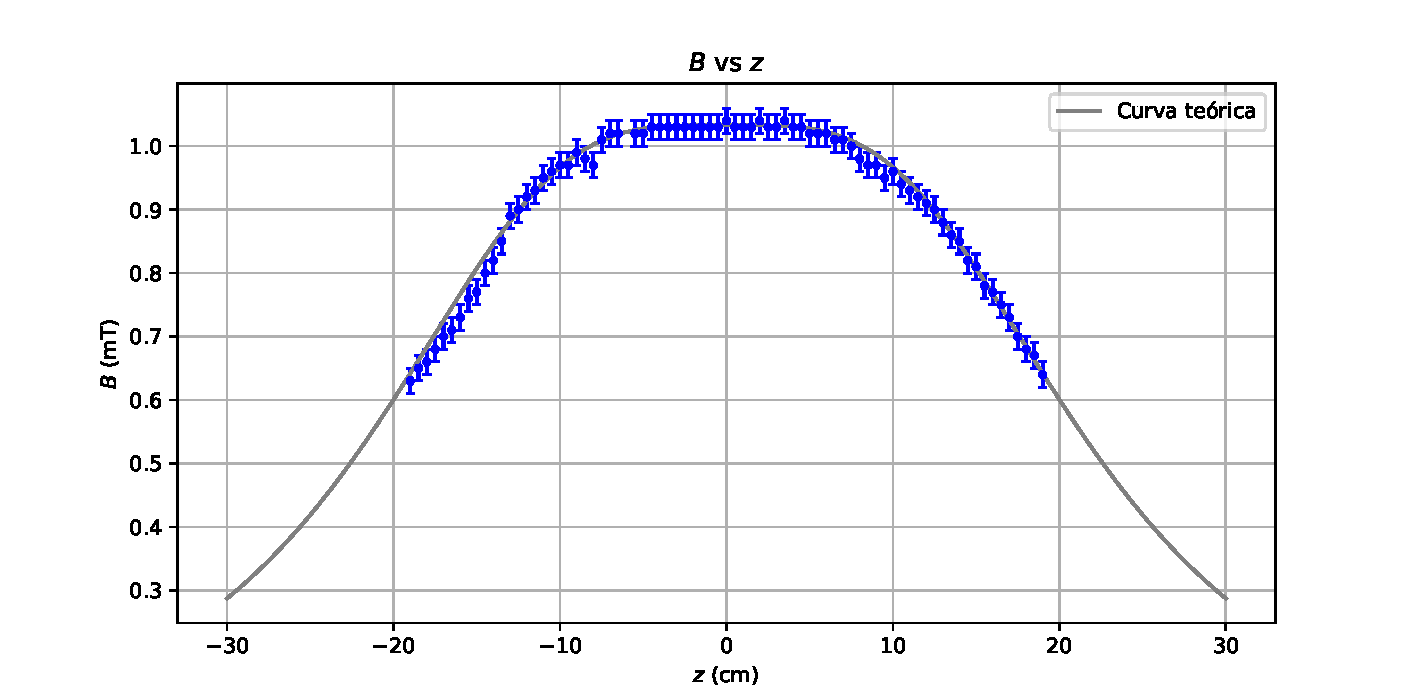
\includegraphics[width=0.7 \linewidth]{1-1-a.pdf}
\end{figure}
\begin{figure}[!htpb]
	\centering
	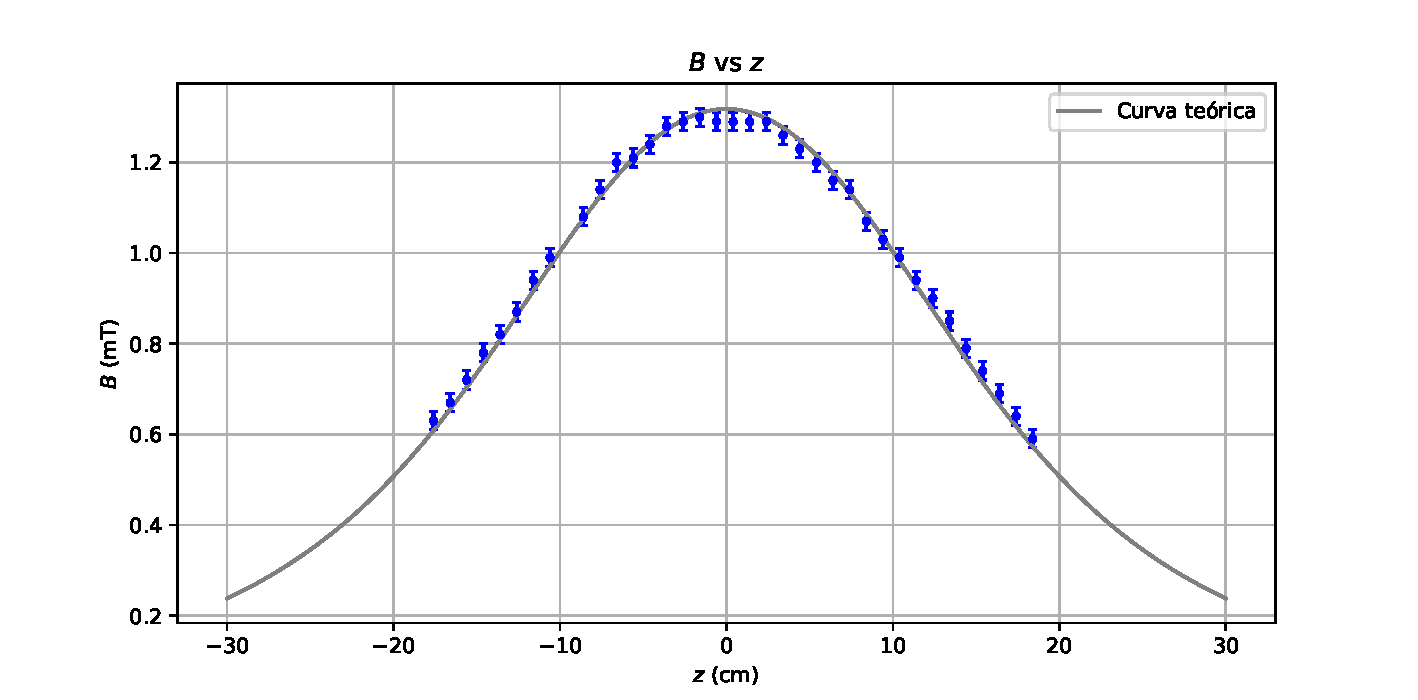
\includegraphics[width=0.7 \linewidth]{1-1-b.pdf}
\end{figure}
\begin{figure}[!htpb]
	\centering
	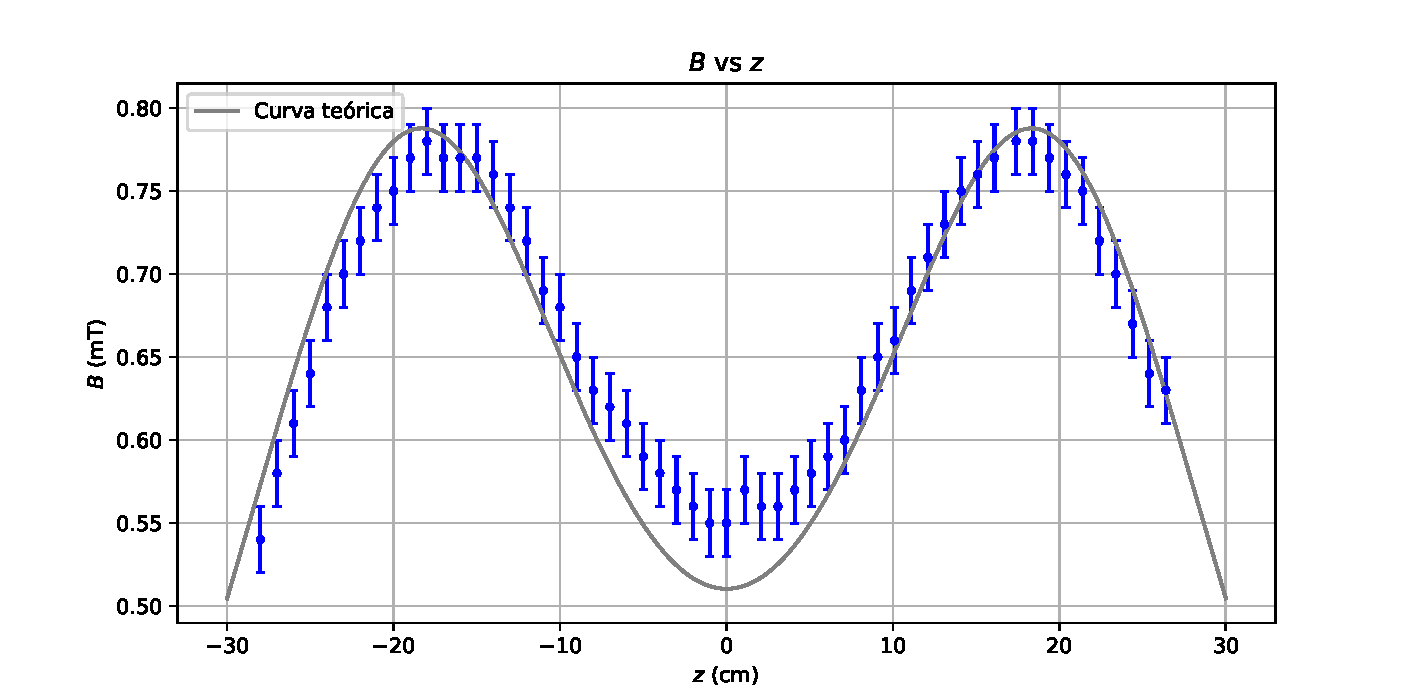
\includegraphics[width=0.7 \linewidth]{1-1-c.pdf}
\end{figure}
\begin{figure}[!htpb]
	\centering
	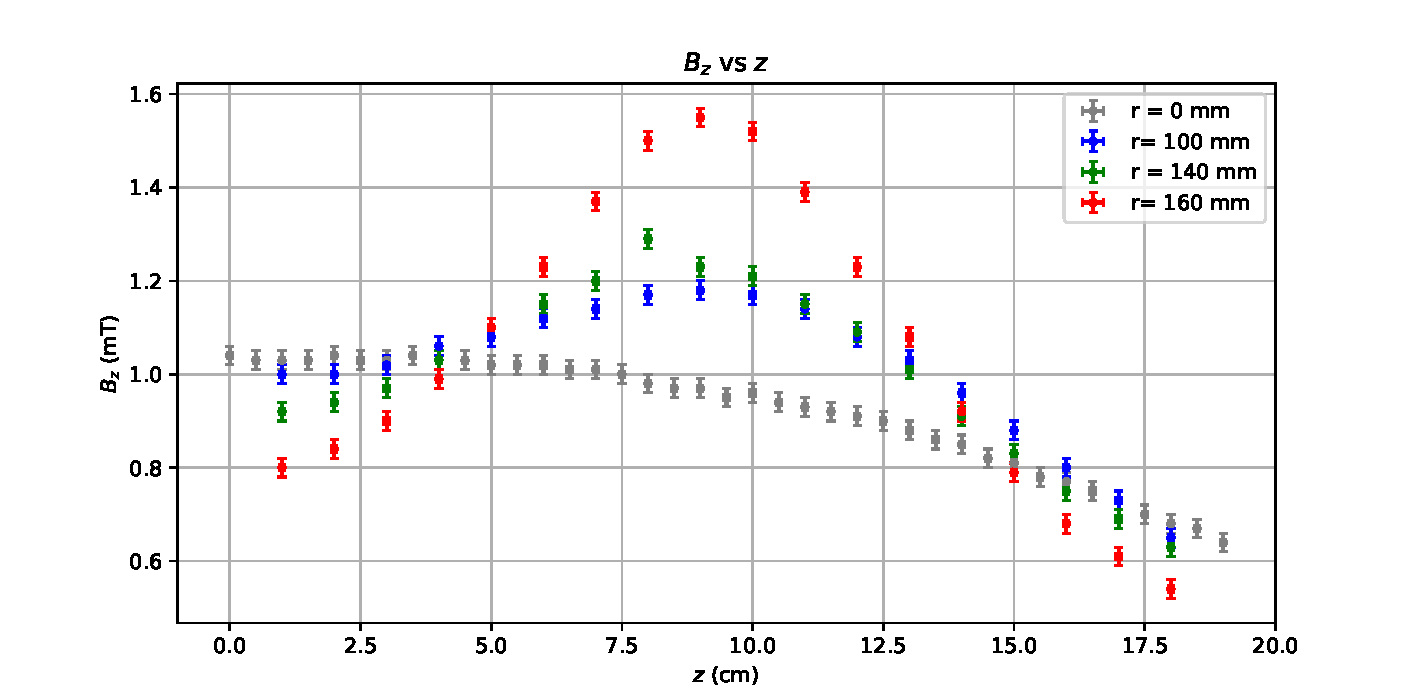
\includegraphics[width=0.7 \linewidth]{1-2.pdf}
\end{figure}
\begin{figure}[!htpb]
	\centering
	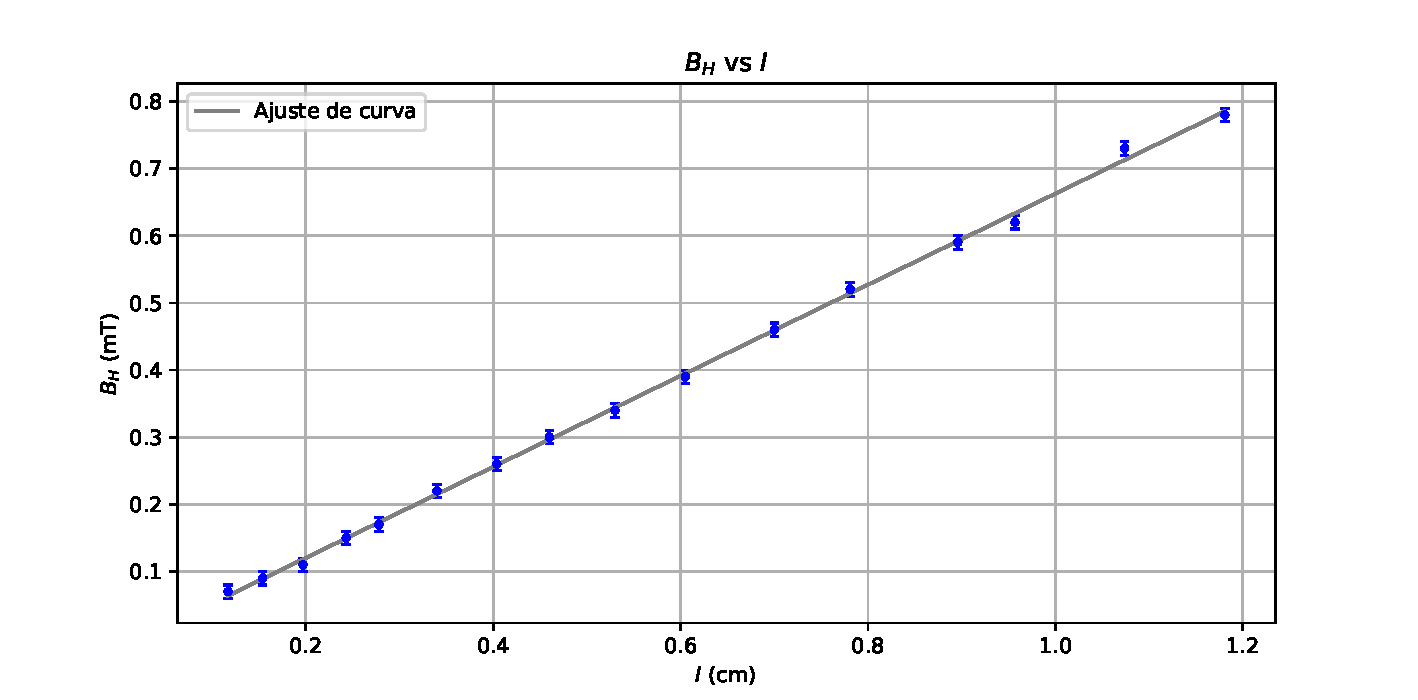
\includegraphics[width=0.7 \linewidth]{2-1.pdf}
\end{figure}
\begin{figure}[!htpb]
	\centering
	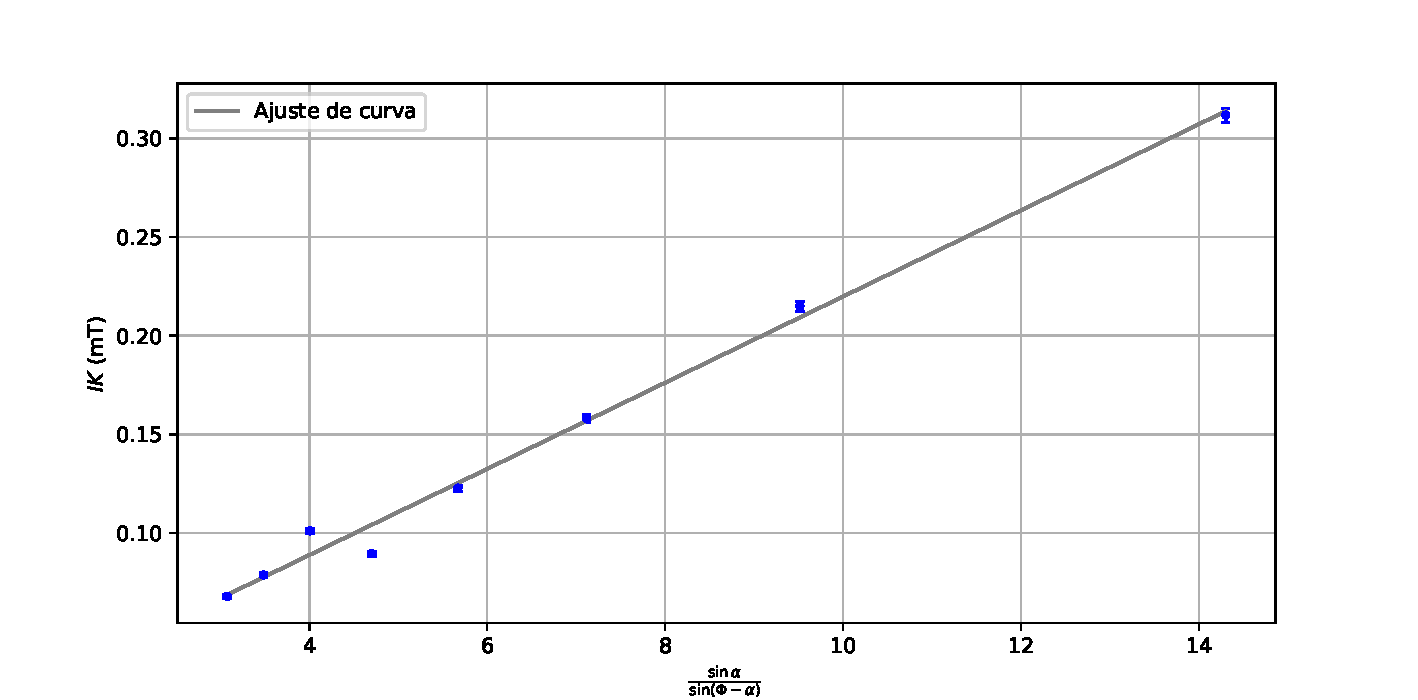
\includegraphics[width=0.7 \linewidth]{2-2.pdf}
\end{figure}
\begin{figure}[!htpb]
	\centering
	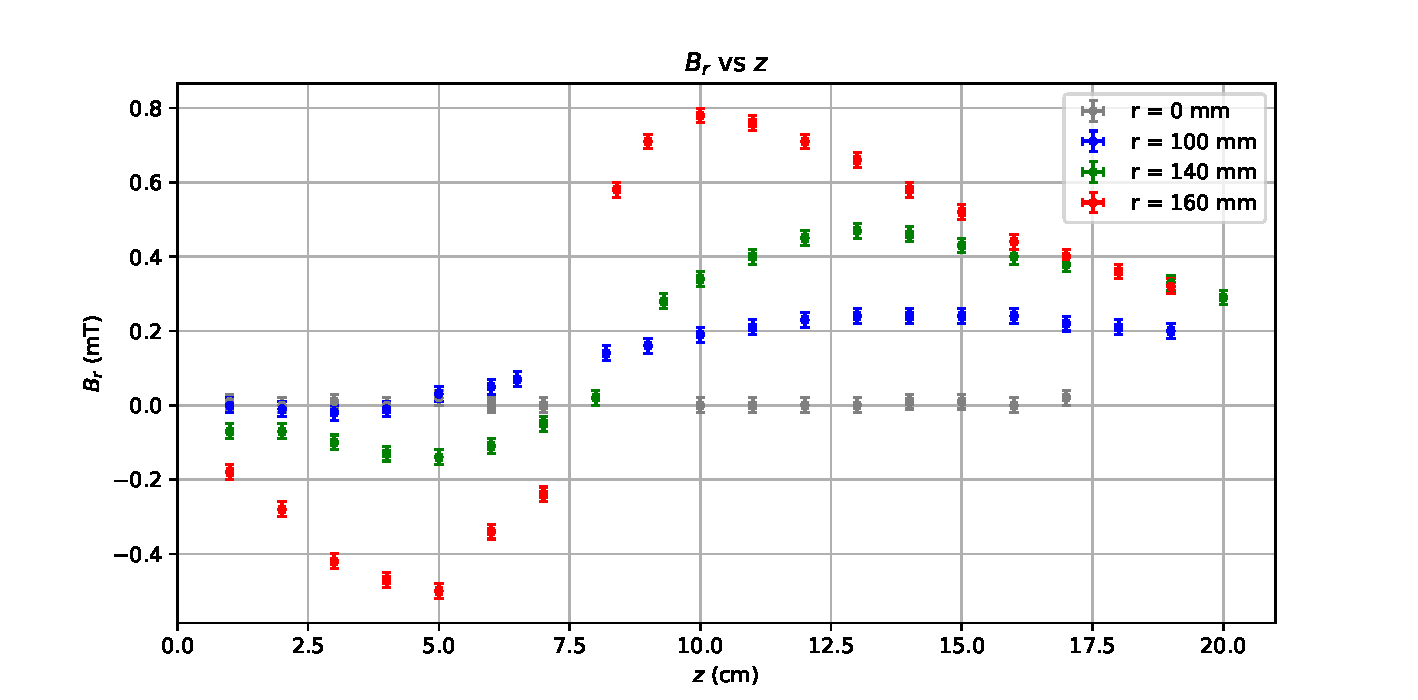
\includegraphics[width=0.7 \linewidth]{1-3.pdf}
\end{figure}
\end{document}
